\documentclass{beamer}
\usetheme{Madrid}

\title{Speech Command Detection in Noisy Environments}
\subtitle{A Deep Learning Approach to Audio Classification}
\author{Team Park: D. Hörtenhuber, O. König, W. Laube}
\institute{JKU \\ MLPC}
\date{\today}

\begin{document}

\begin{frame}
  \titlepage
\end{frame}

\begin{frame}{Introduction}
  \begin{itemize}
    \item \textbf{Objective:}
          \begin{itemize}
          \item Develop a robust speech command detection system for smart home environments.
            \end{itemize}
    \item \textbf{Scope:} 
          \begin{itemize}
    \item Detect commands in noisy, continuous audio streams.
          \end{itemize}
    \item \textbf{Goals:}
      \begin{itemize}
        \item Minimize detection costs.
        \item Evaluate performance in realistic scenarios.
      \end{itemize}
  \end{itemize}
\end{frame}

\begin{frame}{SBasic System Architecture}
  \begin{itemize}
    \item \textbf{Preprocessing:}
      \begin{itemize}
        \item Voice Activity Detection (VAD)
        \item Feature Extraction (MFCCs)
      \end{itemize}
    \item \textbf{Model:}
      \begin{itemize}
        \item CNN with multiple Conv1D layers (later augmented with GRU, LSTM)
        \item Max pooling and dropout for regularization
      \end{itemize}
    \item \textbf{Post-processing:}
      \begin{itemize}
        \item Sliding window approach
        \item Thresholding and command formation
      \end{itemize}
  \end{itemize}
\end{frame}

\begin{frame}{Improvement 1: Hyperparameter Tuning}
  \begin{columns}
    \begin{column}{0.5\textwidth}
      \begin{itemize}
        \item \textbf{Objective:}
        \begin{itemize}
         \item Improve model performance by tuning hyperparameters.
        \end{itemize}
        \item \textbf{Parameters Tuned:}
          \begin{itemize}
            \item Learning rate
            \item Number of layers
            \item Dropout rate
          \end{itemize}
        \item \textbf{Outcome:}
          \begin{itemize}
            \item Increased accuracy
            \item Reduced false positives
          \end{itemize}
      \end{itemize}
    \end{column}
    \begin{column}{0.5\textwidth}
      \begin{figure}
        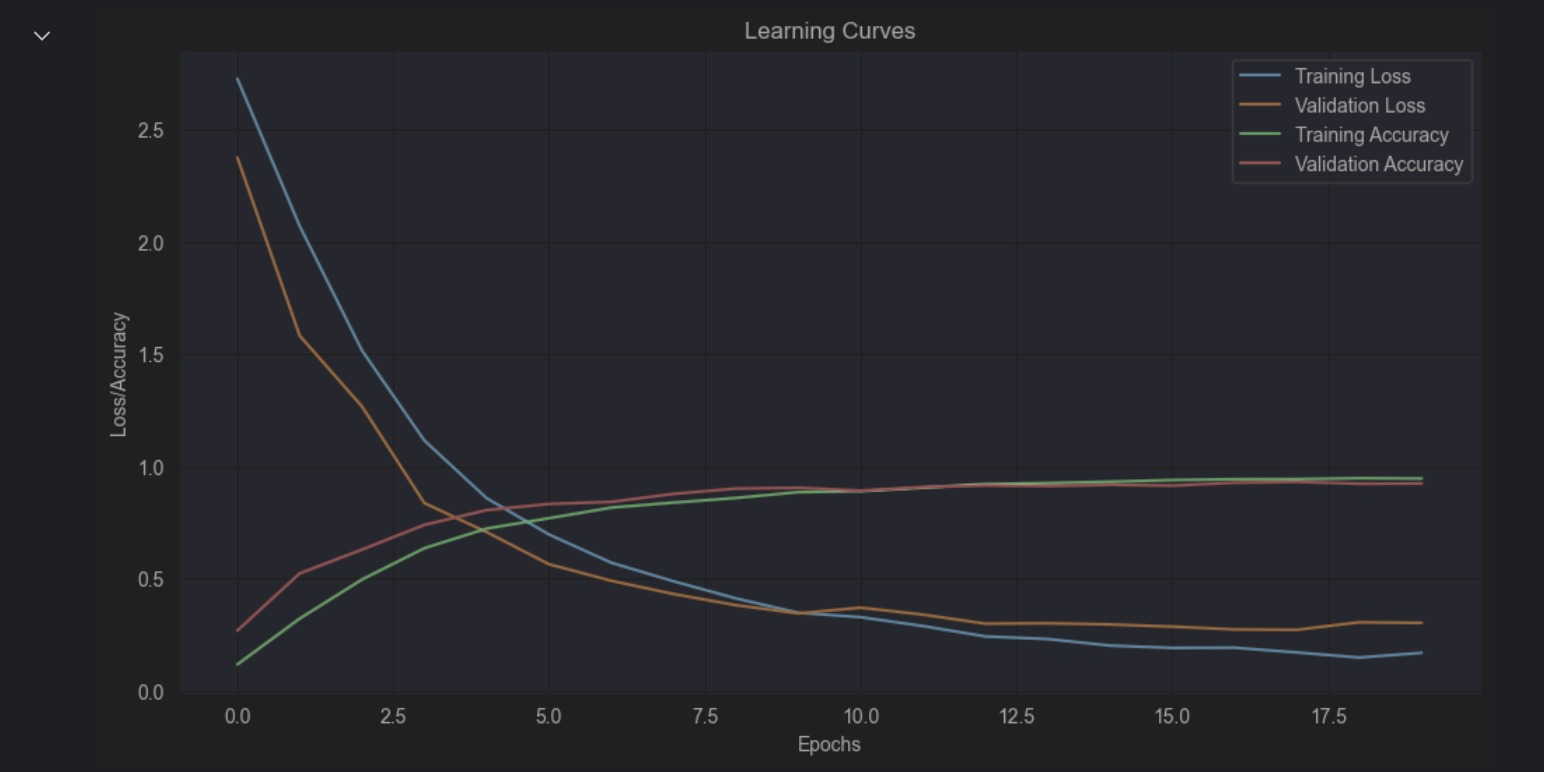
\includegraphics[width=\textwidth]{fig/tuned_learning_curves.jpeg}
        \caption{Model accuracy and loss curves.}
      \end{figure}
    \end{column}
  \end{columns}
\end{frame}

\begin{frame}{Improvement 2: Ensembling}
  \begin{itemize}
    \item \textbf{Objective:}
        \begin{itemize}
        \item     Enhance robustness by combining multiple models.
      \end{itemize}

    \item \textbf{Models Used:}
      \begin{itemize}
        \item Multiple CNNs with different architectures
        \item Ensemble voting mechanism
      \end{itemize}
    \item \textbf{Outcome:}
      \begin{itemize}
        \item Reduced false positives and cross-triggers
      \end{itemize}
      \end{itemize}
\end{frame}

\begin{frame}{Improvement 3: Data Augmentation}
  \begin{columns}
    \begin{column}{0.5\textwidth}
      \begin{itemize}
        \item \textbf{Objective:}
            \begin{itemize}
            \item Improve model robustness to noise and variations.
            \end{itemize}
        \item \textbf{Techniques:}
          \begin{itemize}
            \item Adding background noise
            \item Pitch and speed variations
            \item 3rdParty augemntation data
          \end{itemize}
        \item \textbf{Outcome:}
          \begin{itemize}
            \item Improved performance in noisy environments, reduced false positives
          \end{itemize}
      \end{itemize}
    \end{column}
    \begin{column}{0.5\textwidth}
      \begin{figure}
        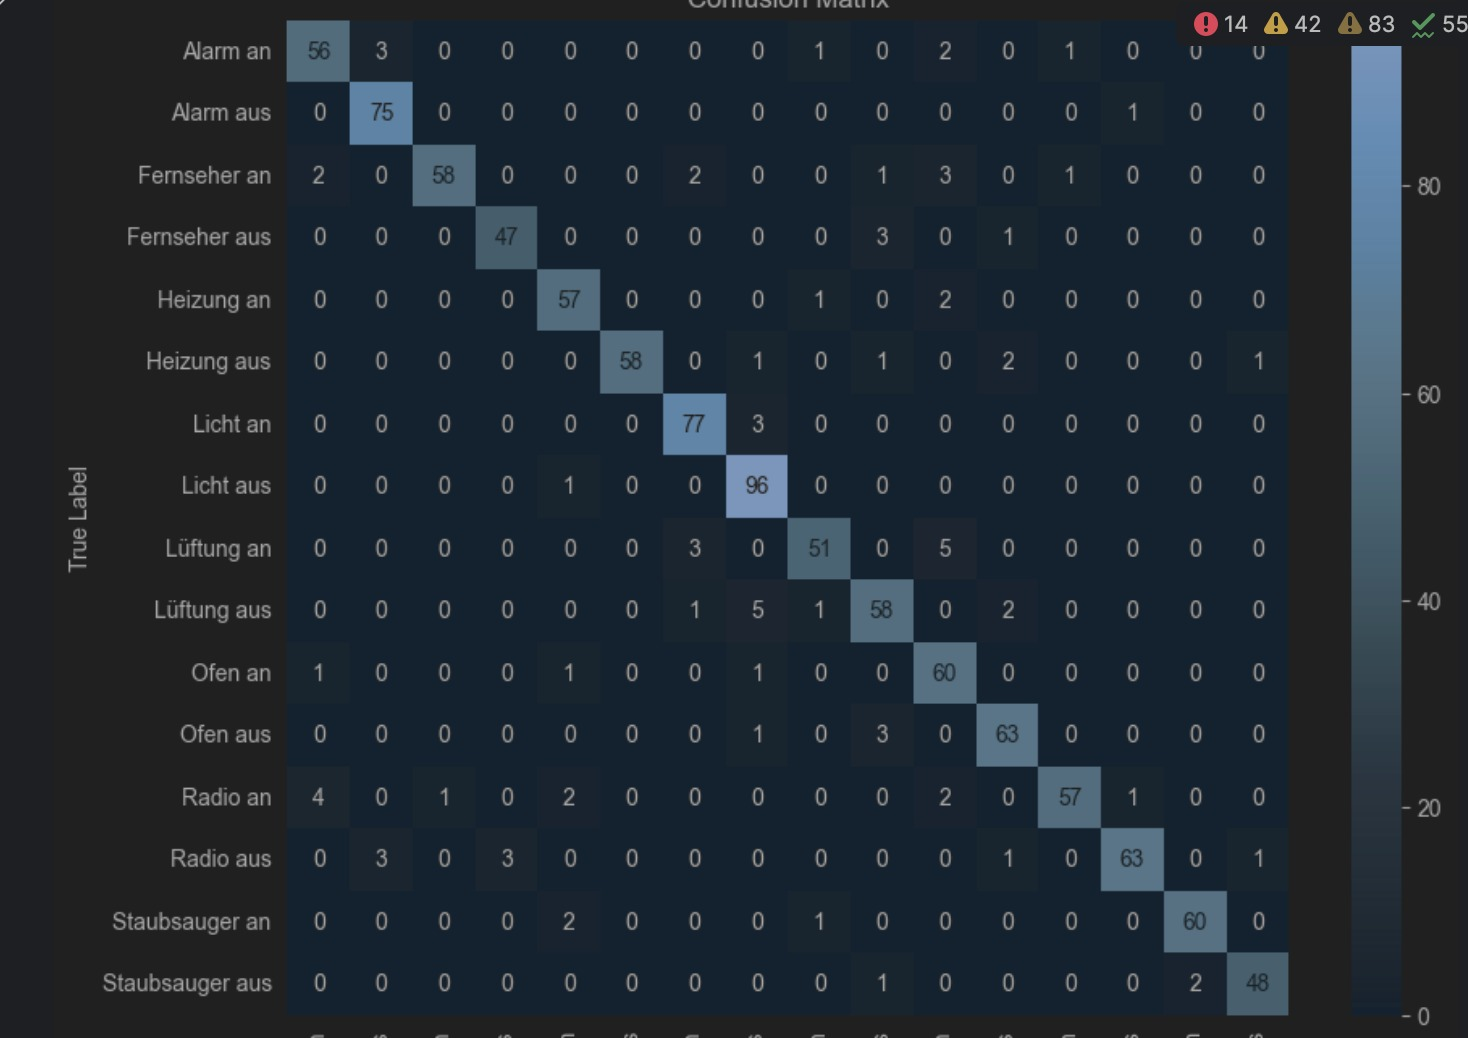
\includegraphics[width=\textwidth]{fig/tuned_heatmap.jpeg}
        \caption{Impact of data augmentation on model performance.}
      \end{figure}
    \end{column}
  \end{columns}
\end{frame}

\begin{frame}{Conclusion and Future Work}
  \begin{itemize}
    \item \textbf{Summary:}
      \begin{itemize}
        \item Developed a robust system for speech command detection
        \item Significant improvements through hyperparameter tuning, ensembling, and data augmentation
      \end{itemize}
    \item \textbf{Future Work:}
      \begin{itemize}
        \item Enhance noise robustness
        \item Incorporate user-specific adaptations
        \item Explore real-time processing capabilities
      \end{itemize}
  \end{itemize}
\end{frame}

\end{document}
